\documentclass[11pt,a4paper]{article}
\usepackage[hyperref]{tto2019}
\usepackage{times}
\usepackage{latexsym}
\usepackage{amsmath}
\usepackage{amssymb}
\usepackage{bm}
\usepackage{tabularx}
\usepackage{graphicx}
\usepackage{tikz}
\usepackage{pgfplots}
\usepackage{tikzscale}
\usepackage{url}
\usepackage{soul}
\usepackage{caption}

\aclfinalcopy % Uncomment this line for the final submission

%\setlength\titlebox{5cm}
% You can expand the titlebox if you need extra space
% to show all the authors. Please do not make the titlebox
% smaller than 5cm (the original size); we will check this
% in the camera-ready version and ask you to change it back.

\newcommand\BibTeX{B\textsc{ib}\TeX}

\title{Parallelizing Deep Neural Network Training}

\author{Trevor Bergstrom \\
  \texttt{trevor.bergstrom@gmail.com} \\\And
  Adam Noack \\
  \texttt{anoack2@uoregon.edu} \\}

\date{12/6/19}

\begin{document}
\maketitle
\begin{abstract}
Deep neural networks (DNNs) are powerful tools that can be used to solve a wide array of tasks. However, it is often the case that a prohibitively large amount of computation is required to train a quality DNN. To combat this issue, the low level matrix operations used to compute the gradients of the error w.r.t. the weights are often parallelized. In addition to the low level operations being parallelized, two DNN training paradigms that rely on parallelization have been proposed: data parallelism and model parallelism. With this paper, we demonstrate the degree to which these different parallelization strategies speed up the training of a deep neural network across a range of tasks and hyperparameters.
\end{abstract}

\section{Introduction}
Over the course of the past decade, deep neural networks (DNNs) have been shown to be useful for solving problems across a number of domains such as image classification \cite{alexnet}, natural language processing \cite{rnn}, and graph data prediction \cite{gcn}. DNNs succeed in these areas where other machine learning algorithms have historically failed because their performance scales well with dataset and network size \cite{dl_book}. Thus practitioners are often incentivized to use the largest possible models with the largest possible datasets. 

The use of large datasets and models does not come without a price, however. The most common training paradigm, \textit{supervised learning}, requires feeding a dataset through a DNN multiple times. Datasets nowadays can be as large as 9 million samples \cite{openimages}, and take up 500GB of space. Therefore, iterating through a dataset even once can take an extremely long time.

Because of the increased demand for high performing DNNs, there has been a recent push to speedup the training process of DNNs. Interestingly, many of the operations involved in the training of DNNs are parallelizable. At a low level, the matrix operations used to pass a single sample through a DNN, calculate the error, and adjust the parameters of the network so that the error will be slightly reduced are highly parallelizable. In addition to vectorizing the low level operations for each sample, two training strategies allow for parallelization at a higher conceptual level: \textit{data parallelism} and \textit{model parallelism}.

Data parallelism refers to the method of distributing the training data across multiple computational resources, where each resource has access to a copy of all of the network's current parameters \cite{beyond_data_model_parallelism}. Each resource passes its portion of the dataset through the network and backpropagates the errors through the network to find the gradients $\nabla_{\theta}f$ for its samples ($\theta$ represents the model's parameters that are learned). The resources must communicate with each other in order to compute the aggregate loss and gradients. Data parallelism typically works best when datasets are high dimensional and large in terms of the number of samples.

Model parallelism, on the other hand, refers to the partitioning of the model across resources \cite{beyond_data_model_parallelism}. A model can be distributed across resources in a variety of ways. Each resource is assigned a portion of the network, but whether that portion is one layer, multiple layers, a portion of a layer, etc., depends on the problem at hand and the model being trained. This method of parallelism is often useful when a network is very large in size.

The base level operations used for these various methods of parallelization are quite numerous, simple, and repetitive. Interestingly, graphics processing units (GPUs) are built for tasks of this nature. Over ten years ago NVIDIA released CUDA, a parallel programming model that makes a GPU's processors available for general purpose computing \cite{cuda}. Since then, GPUs have been shown to be highly useful for speeding up the training time of DNNs \cite{dl_using_gpus, dl_using_gpus2}. 

In this paper we use networks written with CUDA and C++ to:
\begin{itemize}
    \item demonstrate how the vectorization of low level operations speeds up training time using datasets of varying sizes
    \item show how data parallelism with minibatches on single GPU can speed up training time using datasets of varying sizes
    \item investigate the effect of using different reduction techniques on training time
\end{itemize}

% A model can be divided across resources in a few basic ways: each layer of a model can be assigned to a different resource, portions of layers can be assigned to different resources, and different combinations of these two can be used. The architecture of the model largely determines which method of model parallelism is optimal. For example, if a DNN's layers are fully-connected, i.e. each node in layer $l$ passes its value via a weight to each node in layer $l+1$, splitting an individual layer across multiple resources may not be optimal because the amount of communication between resources required to compute the activations for $l$ and feed the activations to $l+1$ would be high because each resource responible for nodes in layer $l$ would have to communicate with each resource responsible for layer $l+1$'s nodes.

% These networks are typically used when dealing with supervised learning problems, and involve learning a model $f: \mathcal{X} \to \mathcal{Y}$, parameterized by $\theta$. Unfortunately, training often involves a massive amount of computation. This at least partially due to the fact that there is a clear positive correlation between the number of parameters in a model and the model's ability to generalize to unseen data (test set accuracy), and also, the number of training samples fed through the model and its generalization ability. However bigger models and larger datasets mean longer training times. Training some models can take days or even months \cite{training_time}. It is a rare few that can afford to wait this long for a model to finish training, so practitioners are often forced to settle for a less than optimal model architecture.

% Interestingly, many of the operations used to train and evaluate DNNs are parallelizable. This is due to the fact that the process of training a DNN involves a large number of simple operations that do not depend on one another. For example, the forward pass through a neural network involves a series of matrix multiplications. When two matrices are multiplied together, the dot products required to compute each element in the resulting matrix are easily parallelizeable. Not every computing architecture is equally great at handling this type of operation, though. For example, typical CPUs have a small number of high performance cores, and while they are great at using their cores to handle a small number of complex tasks, they are not exceptional at tasks that require high throughput. Graphics processing units (GPUs), on the other hand, have a large number of simple, specialized cores. As their name suggests, GPUs were originally designed to render graphics on a screen; the operations used to compute the pixel values in each successive frame are fairly simple but numerous, and GPUs were designed to handle them, specifically. As it turns out, the computations used to generate graphics and the computations used to train machine learning models are similar in some useful ways. Thus, GPUs can be used to speed up the training of DNNs. However, the GPU architecture is different than a CPU's, and without some sort of framework to interact with the GPU, it is difficult to take advantage of.

% In 2007, NVIDIA released CUDA, a parallel programming model, built upon the C language, that represents the first successful attempt to make the GPU's processors easily available for general purpose computing \cite{cuda}. Since then, many papers have shown that massive speedups in training time can be achieved using GPUs \cite{dl_using_gpus}, \cite{dl_using_gpus2}. Today, many of the most popular deep learning platforms on the market such as PyTorch and TensorFlow have CUDA underneath their hoods.

% In addition to parallelizing the matrix operations used to make an inference, calculate gradients, and update a DNN's parameters, other techniques can be used to speed up training time. Two broad classes of these techniques are data parallelism and model parallelism. Methods from each camp can be highly useful for speeding up the training and/or inference time for a model, but the degree to which either is effective depends in large part on the architecture of the model in question. Sometimes using data parallelism or model parallelism is not enough, though.

% Because the rewards associated with developing even marginally more accurate models are often sizeable, a large corpus of work on new parallelization techniques for DNN training and inference has emerged. Many of these works take data and model parallelism and build upon them and mix them in interesting ways. 

% This survey paper first lays out how standard data and model parallelism function in section \ref{background}. Then, in section \ref{works}, some recently published papers that attempt to expand on the basic techniques are summarized.

% \subsection{Data parallelism}
% Broadly speaking, data parallelism refers to the method of distributing the training data  across multiple computational resources where each uses its portion of the data to calculate gradients $\nabla_{\theta}f$, where $\theta$ are the model's parameters that are learned. 

% In most cases, each resource gets a certain number of training \textit{samples} and together the resources can quickly and efficiently work through the dataset. This approach is called batch data parallelism. For example, if the training dataset consists of $n$ samples and there are $m$ resources available, resource 1 can be assigned the first through the $n/m$th sample, resource 2 can be assigned the $n/m + 1$th through the $2n/m$th sample, and so on.

% Sometimes, however, it is optimal to split the individual input samples across multiple resources. In other words, a portion of each input is processed by a separate resource. This is called domain data parallelism. For example, in the case of image processing, each channel of an input can be fed through a copy of the network on a separate resource \cite{model_batch_domain_parallel}.

% As a general rule, data parallelism is efficient when the amount of computation per weight is relatively high.

% \subsection{Model parallelism}
% Model parallelism, on the other hand, refers to the partitioning of a model across resources \cite{beyond_data_model_parallelism}. This method of parallelism is often useful when a network is very large in size. A model can be divided across resources in a few basic ways: each layer of a model can be assigned to a different resource, portions of layers can be assigned to different resources, and different combinations of these two can be used. The architecture of the model largely determines which method of model parallelism is optimal. For example, if a DNN's layers are fully-connected, i.e. each node in layer $l$ passes its value via a weight to each node in layer $l+1$, splitting an individual layer across multiple resources may not be optimal because the amount of communication between resources required to compute the activations for $l$ and feed the activations to $l+1$ would be high because each resource responible for nodes in layer $l$ would have to communicate with each resource responsible for layer $l+1$'s nodes.

% Roughly speaking, model parallelism is efficient when the amount of computation per neuron is high.

\section{Background} \label{background}
In order to understand how the operations involved in the training process of a DNN can be parallelized, it is necssary to understand how training works in the supervised learning paradigm at a few conceptual levels. 
\subsection{Parallelizing the Operations for Stochastic Gradient Descent} \label{training_steps}
Stochastic gradient descent (SGD) performs one forward pass, one loss computation, one backward pass, and one weight update per randomly drawn sample from the training dataset. The computations used to compute these four separate steps can be parallelized. We briefly describe these four operations in order to make the way in which we parallelized them with CUDA clearer.
\begin{enumerate}
    \item A forward pass in which a sample from the dataset is passed through the network. Given a fully connected network $f$, the activation values $\bm{a}_l$ at layer $l$ in the network can be computed using the activation values from the previous layer $\bm{a}_{l-1}$, and the weights connecting layer $l-1$ and layer $l$, $W_l$. This operation is captured by Equation \ref{eq:forward_prop}. 
    \begin{equation} \label{eq:forward_prop}
        \bm{a}_l = \phi(\bm{a}_{l-1} \bm{W}_l + \bm{b}_{l})
    \end{equation}
    \indent The activations for each layer in a network depend on the activations of the layers before it, thus the activations for layer $l$ can only be calculated after the activations for layer $l-1$ have been calculated. So, parallelization cannot happen across multiple layers. Nevertheless, feeding a sample from one layer to the next involves simple matrix multiplication, matrix addition, followed by the application of an activation function $\phi$. Thus each element in the product $\bm{a}_{l-1} \bm{W}_l$ can be computed independent of the rest. Similarly, each element in the vector addition  $\bm{a}_{l-1} \bm{W}_l + \bm{b}_{l}$ can be calculated independently. Furthermore, the application of the activation function $\phi(\cdot)$, which is typically RELU, sigmoid, or Leaky RELU for hidden layers, is an elementwise operation; thus all elements can be worked on concurrently.
    
    \item After a sample is passed from the input layer through the hidden layers to the output layer, the output is compared with label for the sample. This comparison is done using some loss function that quantifies how much the network misses the mark for each sample. A standard loss function for a single sample is the squared error loss function (Equation \ref{eq:se}).
    \begin{equation} \label{eq:se}
        \mathcal{L}(\bm{x}, \bm{y}, \bm{\theta}) = \sum_{j=1}^{c}(\bm{y}_j - f_{\bm{\theta}}(\bm{x})_j)^2
    \end{equation} Here $\bm{x} \in \mathbb{R}^{1 \times m}$ and  $\bm{y} \in \mathbb{R}^{1 \times c}$ where $c$ is the number of classes in the classification problem. $f$ is the network parameterized by $\theta$. As the output space is often greater than $R^1$, the inner subtraction can be sped up by performing an elementwise subtraction between the prediction vector $f_{\bm{\theta}}(\bm{x})$ and the label vector $\bm{y}$. Then elementwise squaring can be applied before a sum reduction occurs on all of the elements.
    
    \item Once a sample is passed through the network and the loss is computed, the loss for the sample is attributed to all of the parameters in the network using backpropagation. Similar to the forward pass's activation values, the gradients for each layer in a network depend on the gradients of the layers after it, thus the gradients for layer $l$ can only be calculated after the gradients for layer $l+1$ have been calculated. However, as with the forward pass, the operations used to backpropagate the error through the network are, at bottom, matrix operations that can be parallelized. The general equation for calculating the error for the weights in layer $l$ if layer $L$ is the output layer involves an application of the chain rule (Equation \ref{eq:bp}).
    \begin{equation} \label{eq:bp}
        \frac{\partial \mathcal{L}}{\partial \bm{W}_l} = \frac{\partial \mathcal{L}}{\partial \bm{a}_L} \cdot 
        \frac{\partial \bm{a}_L}{\partial \bm{z}_L} \cdot 
        \frac{\partial \bm{z}_L}{\partial \bm{a}_{L-1}} \cdot \ldots \cdot
        \frac{\partial \bm{z}_l}{\partial \bm{W}_l}
    \end{equation}
    In particular, for one sample, each partial derivative used to calculate $\frac{\partial \mathcal{L}}{\partial \bm{W}_l}$ is a $1 \times u$ matrix, where $u$ is the number of elements in a given layer. Thus the elements in each matrix multiplication can be calculated in parallel in a manner similar to the forward pass. 
    
    \item After $\frac{\partial \mathcal{L}}{\partial \bm{W}_l}$ and $\frac{\partial \mathcal{L}}{\partial \bm{b}_l}$ has been calculated for each layer $l$, all of the weight and bias matrices can be updated using Equation \ref{eq:update}.
    \begin{equation} \label{eq:update}
    \begin{split}
        \bm{W}_l = \bm{W}_l - \lambda \cdot \frac{\partial \mathcal{L}}{\partial \bm{W}_l} \\
        \bm{b}_l = \bm{b}_l - \lambda \cdot \frac{\partial \mathcal{L}}{\partial \bm{b}_l}
    \end{split}
    \end{equation}
    The parameters for all layers can be updated in parallel. I.e. no layer must wait on any other layer to update its parameters.
\end{enumerate}
\subsection{Data parallelism on a Single GPU}
Whereas SGD operates on single examples, minibatch SGD aggregates the gradients calculated for many samples and updates the parameters of the network based on the aggregated gradients. In doing this, the parameters updates are less noisy and the path taken toward the loss function minima is more direct.

Intriguingly, the forward and backward passes for each sample are calculated using the same set of weights, and the calculations for each sample's forward and backward passes do not depend on any other samples in the minibatch. Thus each sample's forward and backward passes through the network can be calculated in parallel. This is data parallelism. 

Specifically, for the forward pass, the activation vectors $a \in \mathbb{R}^{1\times u}$ at a layer $l$ (where $u$ is the number of neurons in $l$) for the the samples in the minibatch can be calculated using multiple resources in parallel as long as all of the resources have access to the network's weights and biases.

After computing the forward pass for the samples, the resources must communicate with each other in order to find the aggregate loss value for the minibatch.

After the loss computation, the resources can again work on their portions of the minibatch without communicating. Each resource performs backpropagation in order to find the gradients of the loss for its sample(s) w.r.t. to the network's current parameters.

Once each resource has computed the gradients for its sample(s), the resources must communicate with each other again in order to find the average gradients across the minibatch.

With the average gradients available, the resources can work together to update all of the parameters of the network in parallel before receiving the next minibatch and repeating the entire process again.

\subsection{Distributed Neural Network Training}

Further optimizing the training times of deep neural networks can be done by scaling up the hardware used. Modern HPC and machine learning clusters contain multiple GPUs to speed up computation. Effectively using multiple GPUs for neural network training usually consists of one of two distributed parallelism schemes, data parallelism and model parallelism. \cite{LS_DN}

Model parallelism, referenced in the introduction, is effectively used when the model size is large enough that it cannot fit into a single device's memory. Modern data-center GPUs can have up to 32GB of memory, requiring a very large model to overflow it's memory. Though it is not impossible to encounter this issue, it is unlikely as models do not generally benefit from scaling up the the number of parameters past a certain point. Model parallelism suffers from the fact that memory transfers between devices present a significant bottleneck during distributed computing. In model parallelism, each device will preform the forward pass on its layers. Stopping to transfer its resultant outputs to the next device in sequence. This transfer is where the major inefficiency of model parallelism exists. Specifically in the backpropogation step, while each device is performing its work, the other devices are idling, waiting for the forward layers to perform their  . Thus, no real parallelism is at work in the strategy, as multiple devices cannot work at the same time. 

Data parallelism is generally more useful than model parallelism, due to the fact that data-sets are increasing in size at an exponential rate. For example, the OpenImages data-set from Google \cite{openimages} contains more than 9 million images, at over 500GB in total size. Due to the fact that most models require multiple passes over the training data, and the fact that memory transfers present a large bottleneck, it is very beneficial to hold as much of the data-set in memory as close to the compute nodes as possible. 

Further, there exist two forms of data parallelism, synchronous and asynchronous data parallelism. Both require copies of all model parameters to be help on each compute device. \cite{d_parallel}

In basic synchronous data parallelism, each device will compute its outputs for the given batch, preform backpropogation to compute and sum the gradients of the model parameters, as well as the aggregate error for all the training samples in the batch. After each device completes the errors through the batch, they must stop and wait for all other devices to finish their work. Once every device is finished a host will need to gather all of the gradients and aggregate them. The host will need to scatter this aggregated gradient to each device where each device will update the model parameters with the aggregated gradients.

Asynchronous data parallelism involves each device running independently of each other, computing its gradients and updating its model parameters, pushing the parameters to a global parameter server. Each device will communicate with this parameter server before starting the training process, to obtain the most recent parameters. This does not in fact guarantee that each device gets the most recent set of parameters, introducing the problem of stale gradients. This could possibly increase training time and decrease accuracy of the overall model. 

% come rows in a matrix $A_l \in \mathbb{R}^{b \times u}$ where $b$ is the number of samples in the minibatch. Using this approach, the computation for the activation vectors for each of the samples represented by $A_{l+1}$ can be performed in parallel. Thus parallelization can be performed within and across samples.
  
%   Typical loss functions for classification tasks include mean squared error and cross entropy. The error is usually calculated across a number of samples, $n$. The value computed is usually used to inform the practitioner on the DNN's ability to classify samples from the training set. Equation \ref{eq:mse}. 
%     \begin{equation} \label{eq:mse}
%         \mathcal{L}(\bm{X}, \bm{Y}, \bm{\theta}) = \sum_{i=1}^{n}\sum_{j=1}^{c}(\bm{Y}_j^i - f_{\bm{\theta}}(\bm{X})_j^i)^2
%     \end{equation}
%     Here $\bm{X} \in \mathbb{R}^{n \times m}$ and  $\bm{Y} \in \mathbb{R}^{n \times c}$ where
%     $c$ is the number of classes in the classification problem. $f$ is the network parameterized by $\theta$, and given an input $X$ outputs to the space $\mathbb{R}^{n \times c}$. This computation is performed often during training and, while fairly insignificant, involves a number of operations that can be parallelized. As $c$ is often greater than 2, the subtraction between vectors can be sped up by performing an elementwise subtraction between the prediction vector $f_{\bm{\theta}}(\bm{X})^i$ and the label vector $\bm{Y}^i$. Then elementwise squaring can be applied before a sum reduction occurs on all of the elements.
  
% Two, a loss computation in which the outputs produced by the network for each sample are compared with the correct labels using some loss function. Three, a backward pass where the derivative of the error with respect to each parameter in the DNN is calculated. And four, and a parameter update that involves adjusting each parameter in the network using its gradient. In doing this, the network gradually learns a function that maps samples to their correct outputs. 
\section{Methods}
In order to test the degree to which data parallelism on a single GPU speeds up training time, we first wrote a serial neural network written entirely in C++ to serve as a baseline. Then we modified the code so that all of the operations involved in training were performed on a GPU. We did this using  CUDA and C++. If we had had more time, we would have scaled up our data parallelism approach to involve multiple GPUs. 

\subsection{Serial Implementation}
To create a fair baseline on which to evaluate our CUDA implementation of a neural network, we wrote a network using C++. We created a fully connected neural network using purely sigmoid activation functions for each neuron. We purposely did not write a very optimized version of the network because we wanted a maximum running time baseline. The network's matrix operations require row by row iterative computation of resultant values. This also gave us a good starting point from which to write the CUDA version. We were able to identify the operations needed to get each step, described in \ref{training_steps}, for training the network working and correctly learning from a data-set. We created a special matrix container that could hold the data contained in a 2-d matrix in a format for efficient (non-nested) array look ups. 

\subsection{Data Parallelism Implementation Using CUDA}
We began the process of writing the CUDA kernels necessary to train a neural network on a GPU by analyzing the four steps (described in \ref{training_steps}) used to train a DNN. We broke down the steps into operations that could be written as CUDA kernels. We identified a number of matrix operations that would be required including matrix multiplication, matrix transposition, various sum reductions, broadcast addition, elementwise addition, elementwise subtraction, elementwise multiplication, elementwise application of the activation functions and their derivatives, etc. We then wrote kernels for these base level operations. We attempted to write this version as similar to the serial version as to not stray too far from our baseline, the only major difference was replacing iterative matrix operations with CUDA matrix operations. We will cover a few of the design choices we made for the kernels and the implications of these choices in the following subsections. 

\subsubsection{Data Format}
Before diving into the kernels it is worth noting that, as with the serial version, all of the matrices on which we operated (the minibatches of data, the weights, the biases, and the gradients) were stored in row major form in arrays of floats. We made the choice to store the matrices in this form because we predicted that we would be more likely to access individual rows of a given matrix object than columns.

\subsubsection{Writing the CUDA kernels} \label{cuda_kernels}
For the \textbf{matrix multiplication} kernel, we originally thought it might make sense to break the matrix multiplication operation down into two separate kernels: an elementwise multiplication kernel and a sum reduction kernel. The elementwise multiplication kernel could operate on a row from the first matrix and a column from the second matrix. Then the resulting vector could be passed to a sum reduction kernel and reduced to form a single element in the output matrix. However, we noticed that we could combine the elementwise multiplication and the sum reduction into a single kernel, and in doing this, we would not have to write back to main memory more than once per element in the result matrix. Specifically, we could have each block load a row from the left matrix and a column from the right matrix, have each of its threads perform a multiplication between an element from the left matrix's row and an element from the right matrix's column, before loading the product into a shared memory array. After this, a sum reduction could occur in shared memory. Because the maximum number of threads per block is 1,024, this design choice meant that our kernel would be able to perform matrix multiplication between matrices with an inner dimension of up to 1,024. This meant that our minibatch size and the number of neurons in any layer could not exceed 1,024. For the datasets on which we were working this would not be problematic.

We originally considered trying to write the \textbf{matrix transpose} so that the transposition would be placed in the same place in memory as the original matrix, but we realized that unless we did some sort of coordination between blocks, there would be race conditions. Therefore, in order to avoid the race conditions involved with an in-place operation, we wrote the kernel so that it would place the transposed matrix at a new location in memory. 

We wrote an \textbf{all reduce sum reduction} kernel that would take a matrix and sum all of its elements. We wrote it so that, given the number of threads, the minimum number of blocks needed would be used. In particular, we coded the kernel so that each thread from each block could load one element from main memory into shared memory. Then a sum reduction could be performed on the shared memory array by all blocks before writing the sum of each block's portion of the original array to main memory. Then the kernel could be called again, this time with one block, and a second sum reduction could be performed on the results from the first reduction. This reduction was used to calculate the MSE at for each minibatch during training. It can handle reducing arrays with up to $T^2$ elements, where $T$ is the number of threads per block.

In addition to an all reduce sum reduction kernel, we wrote a \textbf{reduce rows} kernel that would sum along each of the columns in a matrix. For this kernel, we decided to assign a block to each column of a matrix, and then have each block peform a sum reduction in shared memory. As with the matrix multiplication kernel, the matrix passed to this kernel needed to have a number of rows less than or equal 1,024. However, this would not be a problem as minibatches are typically smaller than this, and layers with more than 1,024 neurons would not be necessary for our problems.

The kernels written for \textbf{elementwise multiplication, elementwise subtraction, division, the application of activation functions and their derivatives, and the updating of parameters} were fairly similar in that each element in the resulting matrix only depended on the element(s) in the operand matrix(es) in the same relative position. Thus race conditions did not need to be accounted for. These kernels were written so that each thread from each block could calculate one element in the resulting matrix, and the kernel wrappers were written so that each kernel was called with the minimum number of blocks needed to cover all of the elements in the operand matrix(es). This ensured that thread divergence was kept to a minimum. 

We noticed that three of the kernels we wrote relied on \textbf{sum reductions} in shared memory: the all reduce sum reduction kernel, the row reduce sum reduction kernel, and the matrix multiplication kernel. These three kernels would be used often during the training process, so in order to speed up training time, we used sequential addressing and loop unrolling to speed up the reductions. 

In Section \ref{reduction_algos}, we investigate how training time changes when the reduction algorithm used for each of these kernels is altered. In particular, we try four different algorithms covered in the web lecture \cite{choi_reductions}: naive reduction, non-divergent branching reduction, sequential addressing reduction, and a loop unrolled reduction. (1) The naive reduction uses interleaved addressing to reduce the shared memory array. However, because the active threads at each iteration of the reduction are spread across disparate warps, divergence is high. (2) The non-divergent branching algorithm reduces this divergence by clustering the active threads in warps. This means that at each iteration, it is likely that the threads in a given warp are either all working or all idling. (3) The sequential addressing reduction algorithm reduces memory bank conflicts by having each thread at each iteration add two elements from the array separated by a stride that improves memory bandwidth and reduces conflicts. (4) When the size of the relevant portion of the shared memory array has dropped low enough so that it can be handled by a single warp, the synchronization of threads is unnecessary. This is because threads in a warp operate in unison by default. Thus loop unrolling and removing synchronization allows for additional speedup.

\subsubsection{Incorporating the CUDA kernels into our training process}
In order to make the calling of our kernels easier and more understandable, we wrote wrapper functions for each. The wrapper functions use information from the passed matrix objects to determine if the matrices are the correct dimensions for the kernel and have been moved onto the device. Then each of the wrapper functions calls its corresponding CUDA kernel with the matrix objects' data with the minimum number of blocks needed to complete the operation using the number of threads per block that was specified at compile time.

Once the wrapper functions were written, it was relatively straightforward to convert the code we had been using for training the serial neural network into code that would work with the CUDA kernels. For example, many of the for loops over matrices for various operations could be replaced with CUDA kernel wrapper function calls.

The backpropagation function needed to be modified slightly due to the fact that it required matrices to be transposed before matrix multiplication. In order for everything to be performed on the device, we allocated space before training began for temporary matrices that could hold the transposes. After making these modifications and finishing the code for the forward propagation and update functions, we could train the neural network entirely on the device.

\subsection{Distributed Data Parallelism}
Initially, our plan was to use multiple GPUs to train a network using a distributed parallelism approach after completing the data parallelism approach on a single GPU. However, we did not have enough time to complete a working version. 

If we had time, we would have used a \textit{data} parallelism approach for distributed training. Since we are working with fairly simple classification tasks, creating larger models should not result in an increase of performance on the task. Furthermore, we would have implemented a synchronous distributed data parallelism strategy, as it seems to be a more seamless approach to performing network training and should produce better results. 

Synchronous data parallelism requires the compute devices to halt and wait for the other devices to finish forward and backpropagation through their training data. This is done because the average gradients and losses need to be computed so that the model can update its parameters using information gained from all of the training data. The average gradients will need to be computed on a single device,
then passed back to each individual device so that each can update its model parameters with the same average gradients. This gather and scatter process can be accomplished with an AllReduce function, since averaging can be handled by a reduction function. We have available to us two Nvidia GPUs as compute devices, both can run the CUDA GPGPU language. Newer versions of CUDA support device to device memory transfers, which can be used in conjunction with a reduce kernel to compute the average, as long as the remaining memory on the host GPU can support the memory copy. This is how we planned to implement the AllReduce step of the data parallel approach proposed. However, increasing the number of GPUs would involve using the more advanced functionality of the Nvidia Collective Communications Library (NCCL) for many device communication. NCCL supports a GPU AllReduce function.  

\section{Experiments} \label{experiments}
This work benefited from access to the University of Oregon high performance computer, Talapas. All of the following tests were preformed using Talapas hardware.  The serial network was on standard compute nodes, each with 2x Intel-Xenon E5-2690v4 (28 cores total) and 128GB of memory. CUDA tests were run on GPU nodes running 2x Nvidia Tesla K80 with 24GB of VRAM, and 256GB shared memory.  

\subsection{Datasets Used} \label{data_used}
\noindent \textbf{Dataset generation method} Among other things, we wished to determine how varying the size of the dataset would effect training time for the serial and CUDA implementations. Therefore, we needed a way to scale up a dataset without changing the difficulty of the classification task in a large way. Thus we created the following scheme that would allow us to create datasets with an arbitrarily large number of the samples and an arbitrarily large number of features per sample. 

Specifically, given the desired input dimension $m$ (number of features per input), output dimension $c$, and number of samples $n$, the value for the $j$th feature (of $m$ features) in the $i$th sample (of $n$ samples) is $\bm{x}_j^i \sim \mathcal{N}(c\cdot s, \sigma)$, where $c$ is the class label, $s$ controls the spacing between distributions for classes, and $\sigma$ controls the standard deviation of each class's distribution. For all datasets we generated, the number of samples per class was equal.

This process allowed us to create datasets of arbitrary sizes quickly. While the datasets produced using this method should not present much of a learning challenge for even small neural networks, each network being trained must learn to some degree in order to perform well.

\vspace{10pt}
\noindent \textbf{Wholesale Customers Dataset} In order to make sure our networks were able to learn more complex tasks, we trained our networks on the Wholesale Customers Dataset from the UCI Machine Learning Repository \cite{wholesale_cust}. It contains 440 samples, each of which has seven features.

\subsection{Training on the Wholesale Customers Dataset}
To ensure that both the serially trained and CUDA networks were actually capable of learning on a complex problem, we trained the networks on the Wholesale Customers Dataset \cite{wholesale_cust}. Each network consisted of a single hidden layer of five neurons, and ran a batch size of 10 samples per batch. Training was measured by accuracy of the network on a set of samples from the data set. Accuracy was measured by the number of positive samples divided by the total number of samples. Results for this test can be seen in Table \ref{tab:acc}.


\subsection{Training Time Versus Input Dimension}
According to Krizhevsky et al., the larger the ratio of computation to parameters is, the larger the speedup offered by data parallelism will be \cite{one_weird_trick_cnns}. We wished to design an experiment to test this idea. One way to increase the number of computations required per input sample is to increase the dimensionality of the input. Thus we created datasets with varying sizes of inputs. We then trained both the serial and CUDA neural networks on the datasets and observed training time. We held the minibatch size and the number of epochs constant (and therefore the number updates performed, too) across the datasets. It is worth noting that we chose dataset input dimensions in multiples of 32. We did this so that our multiplication and transposition kernels, which were written so that each GPU block operates on a row of data, would not have much thread divergence. Our results are in Figure \ref{fig:input_scaling}.  

\subsection{Training Time Versus Minibatch Size}
In theory, the more samples that can be processed in parallel during each iteration, the better data parallelism will do when compared with the serial implementation. We designed an experiment to test this idea. Given our CUDA implementation, the number of samples that could be processed in parallel (given enough blocks) was as large as our minibatch size. Thus we decided scale up the minibatch size, this time holding the number of steps taken constant. Again, we chose the values for the independent variable in this experiment strategically. Specifically, we chose minibatch sizes in multiples of 32 so that our multiplication kernel, when used in the backward pass for the CUDA network, would have an optimal number of elements to work with, and thread divergence would be kept to a minimum. The results for this experiment are shown in Figure \ref{fig:batch_sz_scaling}.

\subsection{Training Time With Various Reduction Algorithms} \label{reduction_algos}
As explained in Section \ref{cuda_kernels}, three of our CUDA kernels used for training performed sum reductions in shared memory. The kernels that used sum reduction were the matrix multiplication kernel, the all reduce kernel, and the row reduce kernel. Each of these kernels was used quite often during training, especially the matrix multiplication kernel. Therefore, we hypothesized that training time, to a significant degree, would depend on the optimization of these kernels. To test this hypothesis, we conducted the following experiment: Using a dataset with 10,240 samples where each sample has 1,024 features, we varied the reduction algorithms used for the three kernels and measured the amount of time it took for the CUDA neural network to train for 100 epochs. We used four of the algorithms covered in the web lecture \cite{choi_reductions}: naive reduction, non-divergent branching reduction, sequential addressing reduction, and a loop unrolled reduction (these algorithms are briefly explained at the end of Section \ref{cuda_kernels}). Table \ref{tab:reduction_algos} shows the results of this experiment. 

\subsection{Results}
\noindent \textbf{Training on the Wholesale Customers Dataset}
As can be seen in Table \ref{tab:acc}, both the serial network and the CUDA network can learn to correctly classify the samples in the Wholesale Customers Dataset. However, the CUDA neural network takes longer to train than the serial neural network. We hypothesize that although the problem complexity presented by the Wholesale Customers Dataset is higher than the datasets we generated using our method described in Section \ref{data_used}, the input dimensionality is small and the minibatch size usedfor training is also small (we found it to be about 10). This implies that the classification problem that our CUDA network engages in for this dataset is not optimal for data parallelism. Therefore the fact that the CUDA network actually takes longer to train is not much of surprise.

\vspace{10pt}
\noindent \textbf{Input scaling} As can be seen in Figure \ref{fig:input_scaling}, as the dimension of the input samples is increased, the time taken for the serial version grows faster than the time taken for the CUDA version. The amount of time it took for serial and the CUDA version to run through a generated dataset (1,024 samples) 1,000 times was recorded. The CUDA network trains significantly faster when the number of inputs is large; when Num. Inputs is 512, the CUDA network trains 4.27 times faster than the serial network, and when Num. Inputs is 1,024, the CUDA network trains 4.43 times faster than the serial network. 

\vspace{10pt}
\noindent \textbf{Minibatch size scaling} The results in Figure  \ref{fig:batch_sz_scaling} show that, ceterus paribus, the more samples used to calculate the aggregate gradients before updating, the longer training time will take. These results are to be expected. Obviously it will take longer to aggregate the gradients from 512 samples than 32 samples. However, the results in Table \ref{tab:batch_sz_scaling} suggest something more interesting. As suggested in \cite{one_weird_trick_cnns}, as the ratio of the number of computations to the number of parameters grows, the speedup incurred by data parallelism grows. See Table \ref{tab:batch_sz_scaling}. The actual data show exceptions to this rule (e.g. minibatch size of 512 and 1,024), but for the smaller minibatch sizes, the predicted trend holds.

\vspace{10pt}
\noindent \textbf{Training time for various reduction algorithms}
The results in Table \ref{tab:reduction_algos} seem to confirm our hypothesis that sum reduction is used often enough during training that training time is significantly reduced simply by optimizing these reductions. The times required to train the CUDA network for each of the four reduction algorithms (naive, non-divergent branching, sequential addressing, and loop unrolling) follow an expected pattern. The naive reduction algorithm that has high divergence results in the slowest time and is used as the baseline. The non-divergent branching algorithm that reduces the divergence by using the minimum number of warps per iteration performs second best and has a 1.47$\times$ speedup over the naive reduction. The sequential addressing reduction that reduces memory bank conflicts does slightly better than the non-divergent branching reduction and provides a $1.62\times$ speedup over the naive reduction. Finally, unrolling the loop when the relevant portion of the shared array is less than 32 items long incurs a speedup of nearly $2\times$ over the naive algorithm. 

Given the information provided in \cite{choi_reductions}, we expected this to be the case and for all of our other experiments, we used the loop unrolled reduction algorithm in the three kernels that performed sum reductions in shared memory.

\vspace{10pt}
\noindent 
\begin{table} 
\centering
\small
  \begin{tabular}{|c||c|}
    \hline
    Minibatch size & Speedup (between serial and CUDA)\\
    \hline
    \rule{0pt}{2.5ex}$2^5$ & 2.92$\times$\\ 
    \hline
    \rule{0pt}{2.5ex}$2^6$ & 4.52$\times$\\ 
    \hline
    \rule{0pt}{2.5ex}$2^7$ & 7.92$\times$\\ 
    \hline
    \rule{0pt}{2.5ex}$2^8$ & 9.03$\times$\\ 
    \hline
    \rule{0pt}{2.5ex}$2^9$ & 7.62$\times$\\ 
    \hline
    \rule{0pt}{2.5ex}$2^{10}$ & 4.49$\times$\\ 
    \hline
  \end{tabular} \caption{The training time speedup between the serial and CUDA networks at each minibatch size value. This table was generated using the same data used to produce Figure \ref{fig:batch_sz_scaling}.} \label{tab:batch_sz_scaling}
\end{table}


\begin{table} 
\centering
\small
  \begin{tabular}{|c||c|c|}
    \hline
    Reduction Algorithm & Training Time (sec) & Speedup\\
    \hline
    Naive & 45.18 & 1.00$\times$\\ 
    \hline
    Non-div. branching & 30.79 & 1.47$\times$\\ 
    \hline
    Sequential addressing & 27.83 & 1.62$\times$\\ 
    \hline
    Loop unrolled & 23.64 & 1.91$\times$\\ 
    \hline
  \end{tabular} \caption{ The matrix multiplication, sum reduce, and sum reduce rows kernels we wrote rely on sum reductions in shared memory. The effect on training time when using various reduction algorithms for these three kernels is shown above when a CUDA network with one hidden layer is trained on a dataset with 1,024 features and 10,240 samples for 100 epochs. The training times have been averaged over three separate runs. }\label{tab:reduction_algos}
\end{table}

\begin{table} 
\centering
\small
  \begin{tabular}{|c||c|c|}
    \hline
    Network & Accuracy & Training Time (sec)\\
    \hline
    Serial & 80.35 & 1.44\\ 
    \hline
    CUDA & 81.70 & 17.13\\ 
    \hline

  \end{tabular} \caption{ Testing accuracy and training times on both versions of the network. Both were trained using the Wholesale Customers Data-set, a single hidden layer of five neurons, and 440 samples in the data-set. }\label{tab:acc}
\end{table}

% \begin{table} 
% \centering
% \small
%   \begin{tabular}{|c||c|c|}
%     \hline
%     Input Size  & Serial Time (sec) & CUDA Time (sec)\\
%     \hline
%     32 & 47.44 & 17.83\\ 
%     \hline
%     64 & 70.65 & 21.25\\ 
%     \hline
%     128 & 114.25& 29.70\\ 
%     \hline
%     256 & 191.8 & 46.12\\ 
%     \hline
%     512 & 340.14 & 79.73\\ 
%     \hline
%     1024 & 646.09 & 145.95\\ 
%     \hline
%   \end{tabular} \caption{Training times in seconds for each version of the network, for different input sizes. Both networks were  run using the same scaled up data-sets, 32 neurons in a single  hidden layer, 1024 training samples in the data-set, and ran for 1000 epochs.
%  epochs.}\label{tab:input_scaling}
% \end{table}

% \begin{table} 
% \centering
% \small
%   \begin{tabular}{|c||c|c|}
%     \hline
%     Batch Size  & Serial Time (sec) & CUDA Time (sec)\\
%     \hline
%     32 & 0.7 & 0.24\\ 
%     \hline
%     64 & 1.13 & 0.25\\ 
%     \hline
%     128 & 2.06& 0.26\\ 
%     \hline
%     256 & 3.61 & 0.40\\ 
%     \hline
%     512 & 6.02 & 0.79\\ 
%     \hline
%     1024 & 11.14 & 2.48\\ 
%     \hline
%   \end{tabular} \caption{Training times in seconds for each version of the network, ran with different batch sizes. Both networks were trained using the same data-set, 32 inputs, 8 neurons in a single hidden layer, and 1024 training samples in the data-set. The number of steps the network trains was held constant. The number of epochs for every run is computed so the network preforms 1024 weight updates. }\label{tab:batch_scaling}
% \end{table}

\begin{figure}
\flushleft
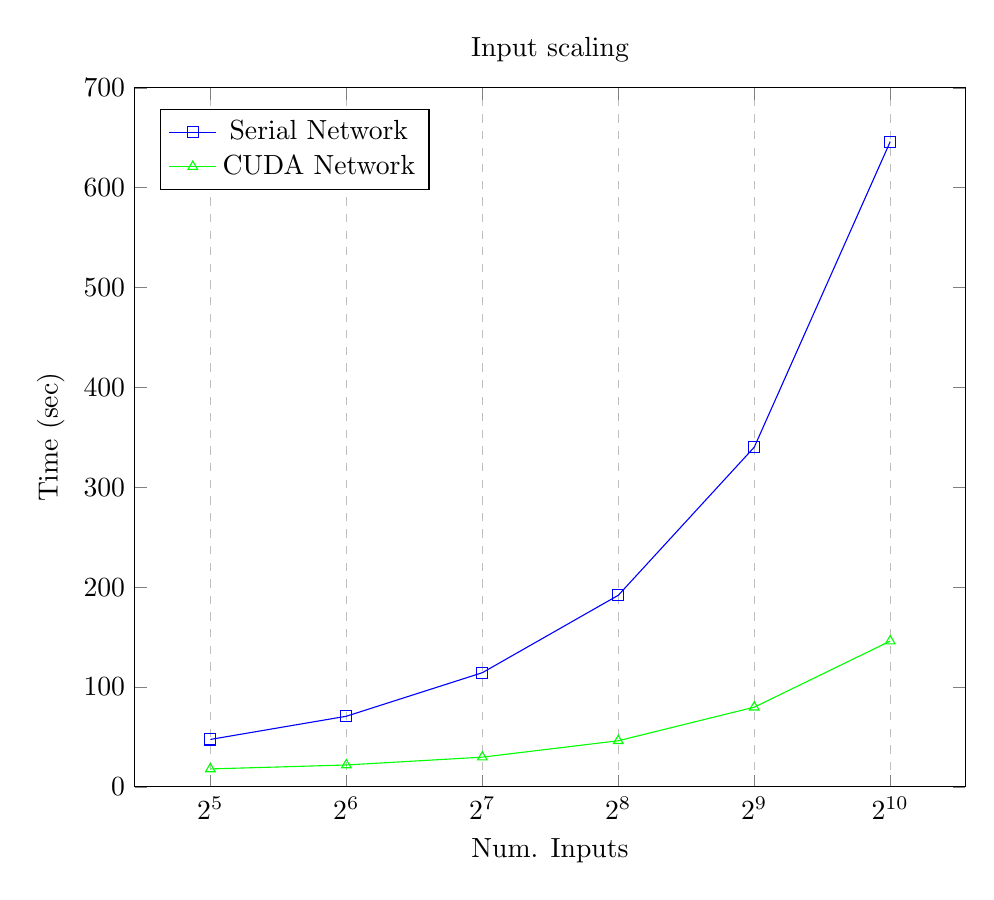
\begin{tikzpicture}
    \begin{axis}[
        width = \linewidth,
        title={Input scaling},
        xlabel={Num. Inputs},
        ylabel={Time (sec)},
        xmax=1500,
        ymin=0, ymax=700,
        xtick={0,32,64,128,256,512, 1024},
        ytick={0,100,200,300,400,500,600,700},
        xmode=log,
        log basis x={2},
        legend pos=north west,
        xmajorgrids=true,
        grid style=dashed,
    ]
    \addplot[color=blue, mark=square,]
        coordinates {
        (32,47.44)(64,70.65)(128,114.25)(256,191.8)(512,340.14)(1024, 646.09)
        };
     \addplot[color=green, mark=triangle,]
        coordinates {
        (32,17.89)(64,21.85)(128,29.7)(256,46.12)(512,79.73)(1024,145.95)
        };
        \legend{Serial Network, CUDA Network}
    \end{axis}
\end{tikzpicture}\caption{Training times in seconds for each version of the network, for different input sizes. Both networks were  run using the same scaled up data-sets, 32 neurons in a single  hidden layer, 1024 training samples in the data-set, and ran for 1000 epochs.
 epochs.} \label{fig:input_scaling}
\end{figure}

\begin{figure}
\flushleft
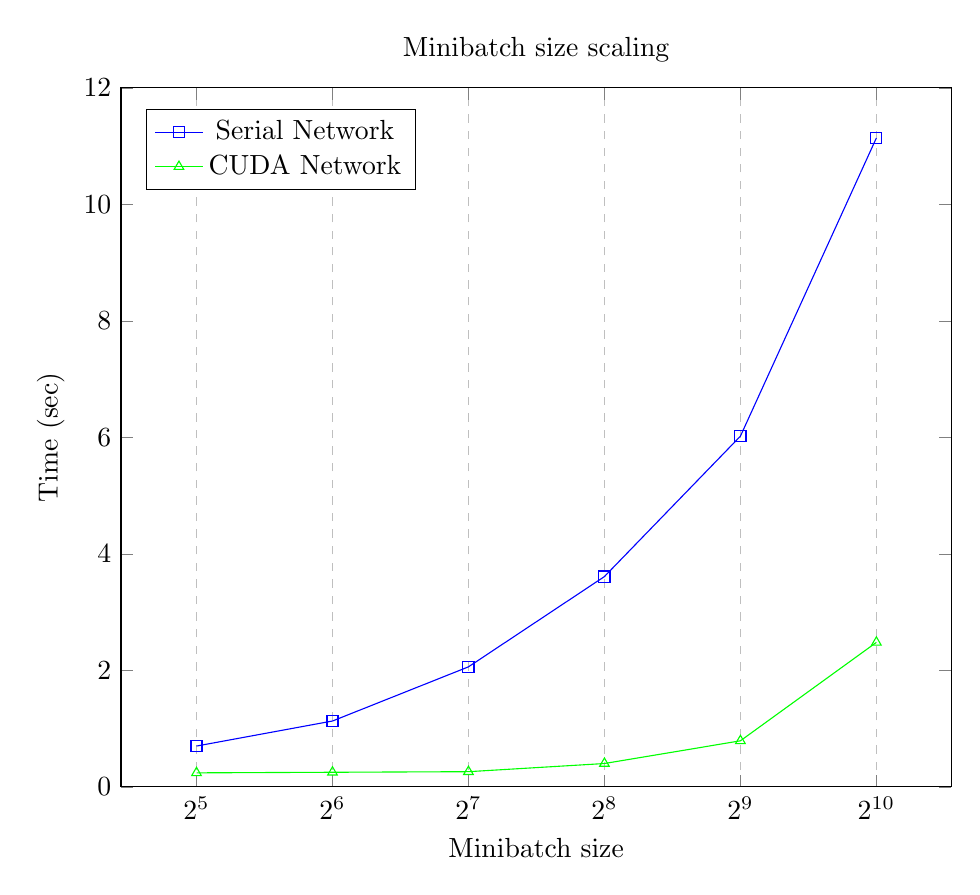
\begin{tikzpicture}
    \begin{axis}[
        width = \linewidth,
        title={Minibatch size scaling},
        xlabel={Minibatch size},
        ylabel={Time (sec)},
        xmax=1500,
        ymin=0, ymax=12,
        xtick={0,32,64,128,256,512, 1024},
        ytick={0,2,4,6,8,10,12},
        xmode=log,
        log basis x={2},
        legend pos=north west,
        xmajorgrids=true,
        grid style=dashed,
    ]
    \addplot[color=blue, mark=square,]
        coordinates {
        (32,0.7)(64,1.13)(128,2.06)(256,3.61)(512,6.02)(1024,11.14)
        };
    \addplot[color=green, mark=triangle,]
        coordinates {
        (32,0.24)(64,0.25)(128,0.26)(256,0.4)(512,0.79)(1024,2.48)
        };
    \legend{Serial Network, CUDA Network}
    
    \end{axis}
\end{tikzpicture}\caption{Training times in seconds for each version of the network, ran with different batch sizes. Both networks were trained using the same data-set, 32 inputs, 8 neurons in a single hidden layer, and 1024 training samples in the data-set. The number of steps the network trains was held constant. The number of epochs for every run is computed so the network preforms 1024 weight updates. }\label{fig:batch_sz_scaling}
\end{figure}

\subsection{Discussion}
The results of these experiments indicate that our CUDA neural network that engages in a data parallelism training approach (1) works correctly (2) trains significantly faster than the serial network under a variety of settings. It is interesting and informative that the CUDA network does not train as quickly as the serial version when the input dimension and minibatch size are small as was the case with the Wholesale Customers Dataset. Thus it is apparent that using a GPU for training does not always guarantee a speedup. There are costs associated with the GPU and whether or not the GPU provides enough of a benefit to outweight those costs depends largely on the dataset, the training approach, and the model.

\section{Conclusion} \label{conclusion}
We were able to create both a serial and CUDA version of a neural network from scratch, without the use of highly optimized linear algebra libraries. Both networks train on a real world data-set. We also created a method of building data-sets that can scale to the size and quality needed for this project.

\subsection{Lessons Learned}

\textbf{The number of variables is high} Getting these networks to work was a big challenge, or at least we thought. It was always hard to tell which portions of our setup needed tweaking. For example, we initially had some problems getting the CUDA network to train, but we were not sure if it was our CUDA kernels or the value of some training hyperparameter that was the problem. We did not completely fix our problem until we tested each individual kernel on small, understandable problems, and got our network to learn on a tiny dataset consisting of just one sample. Therefore we both learned the hard way that building a big, working system is best done by building a small working system and scaling up.

We spent quite a long time writing and tweaking both the CUDA and serial versions of the network, and as a result, we ran out of time to implement a working version of our distributed data parallel approach on multiple GPUs. Though, given the complexity of our problem, a large enough volume of data is probably not necessary to train a model to an acceptable level of accuracy where a data parallel approach would provide a training time speed up. Large data formats such as images for computer vision tasks involving neural networks is a better example of a use case in which data parallelism would provide a significant speed up. The AllReduce, device synchronization, and memory transfer steps provide quite a bottleneck in the training process.

\subsection{Stepping Back and Looking Ahead}
Speeding up the training of deep neural networks is currently a very active area of research. The techniques shown in this project are just a few of the methods available to machine learning and systems engineers for improving training and inference times of neural networks. This is in no way an exhaustive review of what can be done to decrease training time. 

In the coming years, the demand for high performing deep neural networks will continue to grow, particularly as they continue to tackle harder and more realistic problems. Improving model performance can be accomplished with an increasing amount of training data to attempt to cover as many real-world scenarios. Thus, we can expect the size of data-sets to grow exponentially in the coming years. However, without efficient training techniques or highly advanced hardware, it will be infeasible to train models in acceptable time limits. Consequently, the techniques described and analyzed in this report will be needed as deep learning and machine learning continue to affect our lives and drive technological advances.

\bibliography{acl2019}
\bibliographystyle{acl_natbib}

\end{document}
